%%
%%
%%   LaTeX Beamer for ESS Presentation template
%%
%%   Jeong Han Lee, han.lee@esss.se
%%
%%   v0.1 created Monday, Monday, November 23 09:07:19 CET 2015, jhlee
%%
%%

\documentclass[
  9pt
  , table
  , ignorenonframetext
]{beamer}


\usepackage{esspre}
\usepackage{listings}

\meetingname{Timing system training for ICS integrators}
\meetingcity{Lund}
\meetingcountry{Sweden}
\totalpagenumber{\inserttotalframenumber}
%\totalpagenumber{13+}



\title{Timing system training for ICS integrators}
\author{Javier Cereijo Garcia}%\inst{1}}
\institute{
  Integrated Control System Division\\
  \textbf{ESS}, Sweden
}
\date{August 17, 2018}


\begin{document}

\begin{frame}[plain]
  \titlepage
\end{frame}


\begin{frame}{Outline}
    \begin{itemize}
    \item Timing introduction
    \item (E3 introduction)
    \item System configuration
    \item e3-mrfioc2
    \item EVR: basic start-up
    \item EVR: basic configuration
    \item EVR: events and triggers
    \item EVR: backplane clocks
    \item EVR: timestamping
    \item EVR: standalone mode
    \item EVR: inputs
    \item EVG: basic start-up
    \item EVG: basic configuration
    \item EVG: creating events and data
    \item Features in development
    \end{itemize}
\end{frame}

\begin{frame}{Timing introduction (I...)}
  \begin{block}{Principles and requirements}
    \begin{itemize}
    \item Synchronize the operation of the facility
    \begin{itemize}
      \item Accelerator, target, neutron instruments, CF (small extent)
    \end{itemize}
    \item Provide the base frequency of 14 Hz
    \begin{itemize}
      \item Also lower (beam) repetition rates
    \end{itemize}
    \item Provide timestamping to the facility
    \begin{itemize}
      \item Data correlation, EPICS archiving
    \end{itemize}
    \item Provide trigger and clock signals
    \begin{itemize}
      \item With a defined position in an operation sequence
    \end{itemize}
    \item Support post-mortem analysis
    \begin{itemize}
      \item What was the cause of a beam trip?
    \end{itemize}
    \end{itemize}
  \end{block}
\end{frame}

\begin{frame}{Timing introduction (...II...)}
  \begin{block}{Implementation principles}
    \begin{itemize}
    \item A single master unit controls the timing distribution
    \begin{itemize}
      \item Control from one central point
    \end{itemize}
    \item Client units (receivers) act on master’s orders
    \begin{itemize}
      \item No dependency on e.g. computer network traffic
      \item Actions pre-programmed at the receivers
    \end{itemize}
    \item Synchronization to RF
    \begin{itemize}
      \item All timing clocks phase-synchronous to RF (subharmonic)
    \end{itemize}
    \item Distributes "wall-clock" time from the master
      \item Timestamp support in hardware
    \begin{itemize}
      \item Used for data reconstruction and correlation
    \end{itemize}
    \end{itemize}
  \end{block}
\end{frame}

\begin{frame}{Timing introduction (...III...)}
  \begin{columns}
    \begin{column}{.6\textwidth}
      \begin{block}{Structure of the system}
        \begin{itemize}
          \item Master Event Generator (EVG) generates a continuous data stream
          \item The (accelerator) synchronization frequency (of 88 MHz) will be fed into the master event generator and used as the system clock. Event receivers synchronize to that clock.
          \item The 14 Hz operating frequency will be generated by down conversion from RF in the event generator (divide 88.0525 MHz by 6289464 to get 14.00000064 Hz)
          \item All timing sequences, events, etc., generated in hardware
          \item Links work upstream, too
        \end{itemize}
      \end{block}
    \end{column}
    \begin{column}{.5\textwidth}
      \centering
      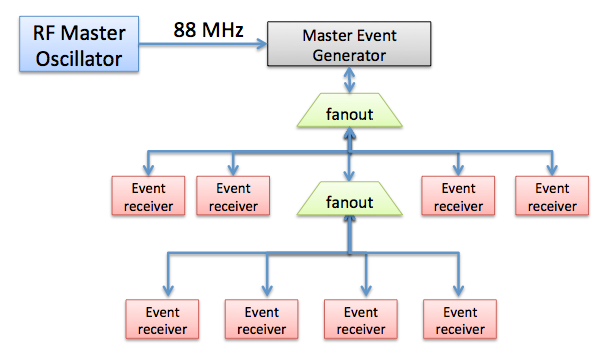
\includegraphics[width=1\textwidth]{./pictures/TimingDistribution.png}
    \end{column}
  \end{columns}
\end{frame}

\begin{frame}{Timing introduction (...IV...)}
  \begin{block}{On-the-wire protocol}
    \centering
    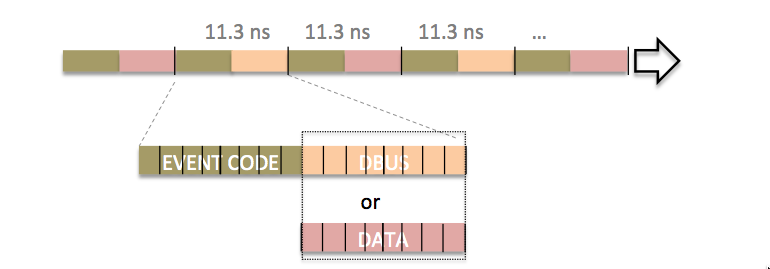
\includegraphics[width=0.6\textwidth]{./pictures/BitStream.png}
    \begin{itemize}
      \item 16-bit "frame" repeating at 88.0525 MHz (11.3 ns), i.e. 352.2 MHz/4
      \item Each frame contains an 8-bit event code and alternating distributed bus/data byte (8 bits).
      \item Distributed bus (DBus) broadcasts eight binary signals which can be output from each Event Receiver. Clocks, status bits, etc.
      \item Event Generator can broadcast arbitrary data (up to 2kB blocks)
      \item Data buffer sent one byte at a time and collected at the receiver(s)
      \item Trigger events and DBUS/Data are independent of each other
    \end{itemize}
  \end{block}
\end{frame}

\begin{frame}{Timing introduction (...V...)}
  \begin{block}{Events, clocks and data}
    \begin{itemize}
      \item Meaning of "event" in this context: signal at a precise time
      \begin{itemize}
        \item Hardware outputs with programmable delay, width, polarity
        \item Event can also trigger software (EPICS) to do actions
        \begin{itemize}
          \item "Collect post-mortem data now", "start counting", etc.
        \end{itemize}
        \item Events can be (synchronously) time-stamped
        \item "Upstream" events: from EVR to EVG (and back)
      \end{itemize}
      \item Clock: a repetitive sequence of pulses
      \begin{itemize}
        \item E.g., a 1 kHz synchronization clock
      \end{itemize}
      \item Data transmission
      \begin{itemize}
        \item Limited amount of data delivered synchronously
        \item For configuration and validation purposes
        \item Still under development (some space for requests)
      \end{itemize}
    \end{itemize}
  \end{block}
\end{frame}

\begin{frame}{Timing introduction (...VI...)}
  \begin{block}{Accelerator cycle}
    \centering
    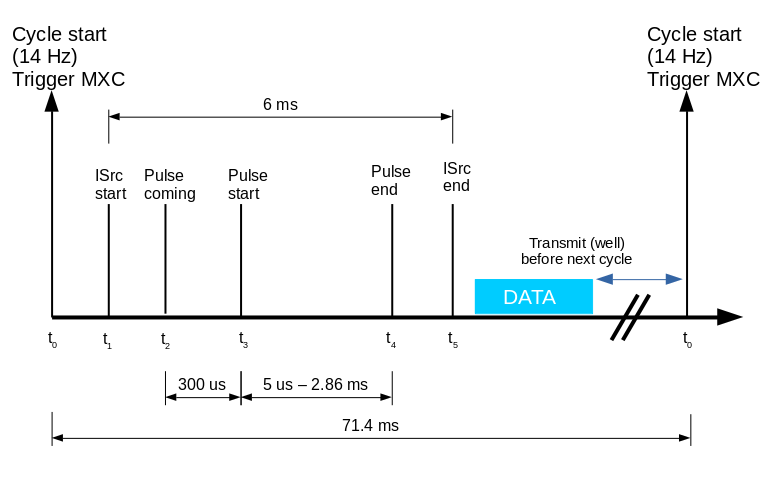
\includegraphics[width=0.5\textwidth]{./pictures/AccCycle.png}
    \begin{itemize}
      \item Pre-programmed sequences repeat at 14 Hz
      \begin{itemize}
        \item Hardware-based (FPGA) sequencer with a RF-synchronous 88 MHz clock
        \item "Programming" can happen in less than a millisecond
      \end{itemize}
      \item "Data", i.e., beam mode, etc., transmitted in parallel
      \begin{itemize}
        \item Contains "plan" for the next cycle: envelope mode, beam/no beam, pulse counter, rep rate, ...
        \item Mode changes require a handshake with BIS
        \begin{itemize}
          \item When mode change is transmitted, timing does not send beam before MPS/BIS gives OK
        \end{itemize}
      \end{itemize}
    \end{itemize}
  \end{block}
\end{frame}

\begin{frame}{Timing introduction (...VII...)}
  \begin{block}{Timing adjustment policy}
    \begin{itemize}
      \item Local delay settings are used for local fine-tuning; adjusting for propagation, processing, etc., delays during commissioning
      \item Pulse length, etc. information in beam data buffer is not for setting the pulse timing locally but for:
      \begin{itemize}
        \item Pulse verification, feed-back/forward, etc.
      \end{itemize}
      \item ”Beam off” will be a dedicated event. A ”gate” signal will be set on with a ”beam on” event and set off with a ”beam off” event
      \begin{itemize}
        \item Central handling of the beam duration, no software activity needed at the (hundreds of ) local receivers (to set the delays)
        \item Actions can be tied to the beam off event, like beam-sync data collection and broadcast
        \item Pulse may be cut short by the timing system. Separate event will allow clean handling of the early pulse abort
      \end{itemize}
    \end{itemize}
  \end{block}
\end{frame}

\begin{frame}{Timing introduction (... and VIII)}
  \begin{block}{Documentation}
    \begin{itemize}
      \item ESS Timing System System Architecture Description - ESS-0088633 - \url{https://chess.esss.lu.se/enovia/link/ESS-0088633/21308.51166.24576.44510/valid}
      \item Data Model Specification for the ESS Timing System - ESS-0225673 - not available yet
      \item Event System with Delay Compensation Technical Reference - \url{http://mrf.fi/fw/DCManual-170209.pdf} (not latest version, ask Javier if interested)
      \item EVR Usage Guide - \url{http://epics.sourceforge.net/mrfioc2/evr-usage.pdf} or \url{https://github.com/epics-modules/mrfioc2/blob/master/documentation/evr-usage.lyx} (lyx version)
      \item Manuals in \url{https://github.com/icshwi/esstex/tree/master/document} (not all of them up to date)
    \end{itemize}
  \end{block}
\end{frame}

\begin{frame}[fragile]{(E3 introduction (I...))}
\begin{lstlisting}[style=termstyle,breaklines=true,basicstyle=\scriptsize]
[iocuser@icslab-ts03 ics_gitsrc]$ git clone https://github.com/icshwi/e3

[iocuser@icslab-ts03 e3-mrfioc2]$ ./e3.bash -t all

[iocuser@icslab-ts03 ~]$ source ~/ics_gitsrc/e3/tools/setenv

Set the ESS EPICS Environment as follows:
THIS Source NAME    : setE3Env.bash
THIS Source PATH    : /epics/base-3.15.5/require/3.0.0/bin
EPICS_BASE          : /epics/base-3.15.5
EPICS_HOST_ARCH     : linux-x86_64
E3_REQUIRE_LOCATION : /epics/base-3.15.5/require/3.0.0
PATH                : /epics/base-3.15.5/require/3.0.0/bin:/epics/base-3.15.5/bin/linux-x86_64:/usr/local/bin:/usr/bin:/usr/local/sbin:/usr/sbin:/home/iocuser/.local/bin:/home/iocuser/bin
LD_LIBRARY_PATH     : /epics/base-3.15.5/lib/linux-x86_64:/epics/base-3.15.5/require/3.0.0/lib/linux-x86_64:/epics/base-3.15.5/require/3.0.0/siteLibs/linux-x86_64

Enjoy E3!
\end{lstlisting}
\end{frame}

\begin{frame}[fragile]{(E3 introduction (... and II))}
\begin{lstlisting}[style=termstyle,breaklines=true,basicstyle=\footnotesize]
[iocuser@icslab-ts03 ics_gitsrc]$ git clone https://github.com/icshwi/essics_scripts

[iocuser@icslab-ts03 ics_gitsrc]$ bash essics_scripts/iocuser_env/iocuser_env_setup.bash clean

[iocuser@icslab-ts03 ics_gitsrc]$ bash  essics_scripts/iocuser_env/iocuser_env_setup.bash install

[iocuser@icslab-ts03 ics_gitsrc]$ bash  essics_scripts/iocuser_env/iocuser_env_setup.bash link

\end{lstlisting}
\end{frame}

\begin{frame}[fragile]{System configuration (I...)}
\begin{lstlisting}[style=termstyle,breaklines=true,basicstyle=\scriptsize]
[iocuser@icslab-ts03 ~]$ lspci
0a:00.0 Signal processing controller: Xilinx Corporation Device 7011
[iocuser@icslab-ts03 ~]$ lspci -s a:0 -vv
0a:00.0 Signal processing controller: Xilinx Corporation Device 7011
	Subsystem: Device 1a3e:132c
	Physical Slot: 1-1
	Control: I/O+ Mem+ BusMaster+ SpecCycle- MemWINV- VGASnoop- ParErr- Stepping- SERR- FastB2B- DisINTx-
	Status: Cap+ 66MHz- UDF- FastB2B- ParErr- DEVSEL=fast >TAbort- <TAbort- <MAbort- >SERR- <PERR- INTx-
	Latency: 0, Cache Line Size: 64 bytes
	Interrupt: pin A routed to IRQ 7
	Region 0: Memory at c0600000 (32-bit, non-prefetchable) [size=256K]
	Capabilities: <access denied>

\end{lstlisting}
\end{frame}

\begin{frame}[fragile]{System configuration (...II...)}
\begin{lstlisting}[style=termstyle,breaklines=true,basicstyle=\scriptsize]
[iocuser@icslab-ts03 ics_gitsrc]$ git clone https://github.com/jeonghanlee/pciids

[iocuser@icslab-ts03 pciids]$ sh replace-pciids.bash

[iocuser@icslab-ts03 pciids]$ lspci -s a:0 -vv
0a:00.0 Signal processing controller: Xilinx Corporation XILINX PCI DEVICE
	Subsystem: Micro-Research Finland Oy MTCA Event Receiver 300
	Physical Slot: 1-1
	Control: I/O+ Mem+ BusMaster+ SpecCycle- MemWINV- VGASnoop- ParErr- Stepping- SERR- FastB2B- DisINTx-
	Status: Cap+ 66MHz- UDF- FastB2B- ParErr- DEVSEL=fast >TAbort- <TAbort- <MAbort- >SERR- <PERR- INTx-
	Latency: 0, Cache Line Size: 64 bytes
	Interrupt: pin A routed to IRQ 7
	Region 0: Memory at c0600000 (32-bit, non-prefetchable) [size=256K]
	Capabilities: <access denied>

\end{lstlisting}
\end{frame}

\begin{frame}[fragile]{System configuration (...III...)}
\begin{lstlisting}[style=termstyle,breaklines=true,basicstyle=\footnotesize]
[iocuser@icslab-ts03 e3-mrfioc2]$ make init

[iocuser@icslab-ts03 e3-mrfioc2]$ make dkms_add

[iocuser@icslab-ts03 e3-mrfioc2]$ make dkms_build

[iocuser@icslab-ts03 e3-mrfioc2]$ make dkms_install

[iocuser@icslab-ts03 e3-mrfioc2]$ make setup

\end{lstlisting}
\end{frame}

\begin{frame}[fragile]{System configuration (... and IV)}
\begin{lstlisting}[style=termstyle,breaklines=true,basicstyle=\scriptsize]
[iocuser@icslab-ts03 e3-mrfioc2]$ systemctl status dkms
● dkms.service - Builds and install new kernel modules through DKMS
   Loaded: loaded (/usr/lib/systemd/system/dkms.service; enabled; vendor preset: enabled)
   Active: active (exited) since Fri 2018-08-17 10:28:19 CEST; 57s ago
     Docs: man:dkms(8)
  Process: 793 ExecStart=/bin/sh -c dkms autoinstall --verbose --kernelver $(uname -r) (code=exited, status=0/SUCCESS)
 Main PID: 793 (code=exited, status=0/SUCCESS)
    Tasks: 0
   CGroup: /system.slice/dkms.service

Aug 17 10:28:18 icslab-ts03 systemd[1]: Starting Builds and install new kernel modules through DKMS...
Aug 17 10:28:19 icslab-ts03 systemd[1]: Started Builds and install new kernel modules through DKMS.
\end{lstlisting}
\end{frame}

\begin{frame}{e3-mrfioc2}
  \begin{itemize}
    \item \url{https://github.com/icshwi/e3-mrfioc2/}
    \item Cmds: startup scripts
    \item Opi: community opis with ESS naming (check readme for opis up to date)
    \item Template: substitutions files
    \item Installation path: /epics/base-3.15.5/require/3.0.0/siteMods/mrfioc2/2.2.0-rc2/db/
  \end{itemize}
\end{frame}

\begin{frame}[fragile]{EVR: basic start-up}
\begin{lstlisting}[style=termstyle,breaklines=true,basicstyle=\scriptsize]
### Load the mrfioc2 module ###
require mrfioc2,2.2.0-rc2

### Define several needed macros ###
epicsEnvSet("IOC", "TRAINING")
epicsEnvSet("DEV1", "EVR1")
epicsEnvSet("MainEvtCODE" "14")
epicsEnvSet("HeartBeatEvtCODE"   "122")
epicsEnvSet("ESSEvtClockRate"  "88.0525")

### Register the EVR with the IOC and load the database ###
mrmEvrSetupPCI("$(DEV1)",  "0a:00.0")
dbLoadRecords("evr-mtca-300u-ess.db","EVR=$(DEV1), SYS=$(IOC), D=$(DEV1), FEVT=$(ESSEvtClockRate)")

### Needed with software timestamp source w/o RT thread scheduling ###
var evrMrmTimeNSOverflowThreshold 100000


iocInit()

### Set delay compensation to 70 ns, needed to avoid timesptamp issue ###
dbpf $(IOC)-$(DEV1):DC-Tgt-SP 70

\end{lstlisting}
\end{frame}

\begin{frame}[fragile]{EVR: basic configuration}
\begin{lstlisting}[style=termstyle,breaklines=true,basicstyle=\scriptsize]
[iocuser@icslab-ts03 cmds]$ iocsh.bash startup_EVR.cmd

TRAINING-EVR1:Link-Sts

TRAINING-EVR1:Link-Clk-SP

TRAINING-EVR1:Link-Clk-I

TRAINING-EVR1:Cnt-LinkTimo-I

TRAINING-EVR1:FwVer-I

\end{lstlisting}
\end{frame}

\begin{frame}[fragile]{EVR: events and triggers}
\begin{lstlisting}[style=termstyle,breaklines=true,basicstyle=\scriptsize]
TRAINING-EVR1:EvtECnt-I

TRAINING-EVR1:DlyGen0-Evt-Trig0-SP

TRAINING-EVR1:DlyGen0-Width-SP

TRAINING-EVR1:OutFPUV00-Src-SP

TRAINING-EVR1:OutFPUV00-Src-Pulse-SP
TRAINING-EVR1:OutFPUV00-Src-DBus-SP
TRAINING-EVR1:OutFPUV00-Src-Scale-SP

\end{lstlisting}
\end{frame}

\begin{frame}{EVR: backplane clocks}
\end{frame}
\begin{frame}{EVR: timestamping}
\end{frame}
\begin{frame}{EVR: standalone mode}
\end{frame}
\begin{frame}{EVR: inputs}
\end{frame}
\begin{frame}{EVG: basic start-up}
\end{frame}
\begin{frame}{EVG: basic configuration}
\end{frame}
\begin{frame}{EVG: creating events and data}
\end{frame}
\begin{frame}{Features in development}
\end{frame}

\begin{frame}{Features in development (I...)}
  \begin{block}{Supercycle}
    \begin{itemize}
      \item Supercycle: a predefined sequence of machine cycles:
      \begin{itemize}
        \item Timing pattern
        \item Beam parameter (data)
      \end{itemize}
      \item Cycles are pre-configured (with a control-room application)
      \item E.g., a supercycle for:
      \begin{itemize}
        \item 1 Hz operation must have 1 cycle with beam, 13 cycles without beam
        \item 0.1 Hz: 1 cycle with beam,  139 cycles without beam
      \end{itemize}
      \item Editor application (to be developed) allows to define
      \begin{itemize}
        \item pulse length (timing events in HW sequencer)
        \item beam current (iris change, probably not between cycles)
        \item pulse delay (within 2.86 time window, in sequencer)
        \item beam destination (in data buffer)
        \item beam mode (in data buffer)
        \item etc.
      \end{itemize}
      \item Concept still needs refinement
    \end{itemize}
  \end{block}
\end{frame}

%\begin{frame}{}
%\end{frame}

\begin{frame}{Questions?}
  \begin{center}
    {\Huge Questions?}
  \end{center}
\end{frame}



% \begin{frame}{EPICS Environment}
%   There is no generic EPICS environment, and each lab has its own environment historically. Historically, many labs use more than one EPICS release and drivers should be built for all EPICS releases in parallel
%   \begin{block}{Loadable Driver Module (LDM) at PSI}
%     \begin{itemize}
%     \item Build drivers for multiple releases of EPICS, and load drivers dynamically from startup script.
%     \item is used to run PSI machine since 2005, which is the first presentation in the community.
%     \end{itemize}
%   \end{block}
%   \begin{exampleblock}{ESS EPICS Environment}
%     \begin{itemize}
%     \item has been evolved from LDM in cooperation with Dirk Zimoch at PSI.
%     \item provides a collection of scripts to develop, build, and deploy an EPICS IOC.
%     \item provides customized solutions to run different configurations at the same time and in the same machine, to test next releases of IOCs independently, and to switch the old and new versions of an IOC easily and quickly.
%     \end{itemize}
%   \end{exampleblock}
% \end{frame}
%
%
% \begin{frame}{Motion Control - MPS integation}
%   \begin{columns}
%     \begin{column}{.6\textwidth}
%       \begin{block}{MCU 1013 - Single Axis MPS version}
%         \begin{itemize}
%         \item CPU, couplier, linear stage, INC encoder, redundant switches
%         \item Motion control with an Open Source EtherCAT master, which is being developed by ICS and the motion group at ESS
%         \item Based on the open source EtherCAT technology
%         \item The Open Source EtherCAT master (www.etherlab.org) can run on Linux
%         \item  No software licences
%           %%   \begin{itemize}
%           %%   \item EtherCAT hardware have rather high performance
%           %%   \item The Open Source EtherCAT master (www.etherlab.org) can run on Linux
%           %%   \item No software licences
%           %%   \item MCAG group also evaluates an industrial control system called TwinCAT (soft controller running under Windows operating system only) with EtherCAT hardware and the same hardware can be used with this open source approach
%           %%   \item ICS is also using open source ethercat master (www.etherlab.org) for sampling analog and digital signals to EPICS.
%           %%   \end{itemize}
%         \end{itemize}
%       \end{block}
%     \end{column}
%     \begin{column}{.5\textwidth}
%       \centering
%       \includegraphics[width=1\textwidth]{./pictures/motion-ws-dual-axis.eps}
%
%     \end{column}
%     \end{columns}
% \end{frame}
%
%
% %% \begin{frame}{Interface Description \textbf{iff} FW in FE, BE, or Both}
% %%   \begin{exampleblock}{Example : Communication}
%
% %%   The Supplier shall provide the required interface to control the XXX remotely. The remote communication protocol shall be compliance with the ESS ICS Standard and the remote communication could be performed through Ethernet networks. The Ethernet interface provides the ability to use TCP socket connection and to fulfill the standard Ethernet attached devices requirements as follows:
%
% %% \begin{itemize}
% %% \item Ethernet-attached devices shall be compatible with a 1 Gb/s network
% %% \item Ethernet-attached devices shall operate at a minimum network speed of 100 Mb/s
% %% \item Ethernet-attached devices shall obtain their network address either through static address configuration or DHCP.
% %% \item Ethernet-attached devices shall include a Standard RJ-45 modular connector
% %% \item Cables should be wired by the Industry Standard Pin-out
% %% \end{itemize}
% %% \end{exampleblock}
% %% \end{frame}
%
%
% \begin{frame}{Questions}
%   In mathematics the art of proposing a question must be held of higher value than solving it.\\
%   \begin{flushright}
%     Georg Cantor
%   \end{flushright}
%
%   It is not enough for me to ask the question; I want to know how to answer the one question that seems to encompass everything I face: What am I here for?
%    \begin{flushright}
%     Abraham Joshua-Heschel
%    \end{flushright}
%
%    Computers are useless. They can only give you answers.
%    \begin{flushright}
%      Pablo Picasso
%    \end{flushright}
%
% \end{frame}
%
%
%
% %% \begin{frame}{ICS Control System Fact}
% %%   \begin{exampleblock}{until 2016.06}
% %%     \begin{itemize}
% %%     \item \includegraphics[width=0.06\textheight]{./pictures/epics_logo.eps}~ \textbf{EPICS}, and ESS EPICS Environment
% %%     \item \includegraphics[width=0.05\textheight]{./pictures/centos-emboss.eps} ~ CentOS 64bit for OS (7.1  1503)
% %%     \item \includegraphics[width=0.08\textheight]{./pictures/git_logo.eps}~ for sources version control
% %%     \item Event System : MRF EVG/EVR boards (cPCI, PCIe, VME, MTCA, etc)
% %%     \item Siemens S7 PLC
% %%     \item Control System Studio for OPI
% %%     \end{itemize}
% %%   \end{exampleblock}
% %%   \end{frame}




%% \begin{frame}
%%   \frametitle{A Page for a picture}
%%   \includegraphics[width=\columnwidth]{./pictures/xchicane.eps}
%% \end{frame}


% \begin{frame}[plain]
%   \begin{center}
%     {\LARGE ¡Gracias!}\\\vspace{6mm}
%     {\LARGE Tack!}  \\\vspace{6mm}
%     {\LARGE 감사합니다!}\\\vspace{6mm}
%     {\LARGE Thank you!}  \\\vspace{6mm}
%     {\LARGE Dankesch\"on!} \\\vspace{6mm}
%     {\LARGE Grazie!}  \\\vspace{6mm}
% %            {\LARGE Merci!}\\\vspace{6mm}
%     {\LARGE \smiley }
%   \end{center}
% \end{frame}


\end{document}
